\section{Шаги удаления и геометрическое продвижение}
Пусть $Q=\operatorname{conv}(\mathcal A)$ для конечного множества
атомов. Поддерживается представление $x=\sum_{a\in S}\lambda_a a$
с положительными весами, сумма которых равна единице. Помимо полного
FW-атома $s$, выбирается
$v\in\arg\max_{a\in S}\inner{\nabla f(x)}a$.
Из направлений $s-x$ и $x-v$ используется направление с большим
зазором; при равенстве выбирается FW. Его зазор $g$ удовлетворяет
$g\ge G\ge U$, а норма не превосходит $D$. Допустимая верхняя граница
шага равна $1$ для FW и $\lambda_v/(1-\lambda_v)$ для шага удаления;
при одном активном атоме выбирается FW. Применяется та же проверка
с делением и умножением оценки на два и
$\alpha=\min\{a_{\max},g/(L\norm d^2)\}$.
Это стандартный FW с шагами удаления (AFW)~\cite{lacostejaggi,pedregosa}.
В сертификате по-прежнему используется полный FW-зазор. Поиск по
активному множеству является дополнительной работой и учитывается
отдельно от полных вызовов LMO.

Шаг удаления на допустимой верхней границе удаляет атом; назовём
его максимальным удалением, а остальные шаги — хорошими.
Если было $m$ хороших обновлений, число максимальных удалений не
превосходит числа FW-обновлений плюс $|S_0|-1$, откуда
\begin{equation}\label{eq:dropcount}
 N\le2m+|S_0|-1.
\end{equation}
Действительно, FW добавляет не более одного атома, максимальное
удаление убирает один, а активное множество остаётся непустым.
Полные FW-шаги могут убирать больше атомов и лишь улучшают оценку.

\begin{theorem}[Выпуклая сертификатная оценка AFW]\label{thm:afw}
При $J,P$ из теоремы~\ref{thm:fw} AFW достигает
$U_N\le\varepsilon$ за
\[
 N\le2\left[P+\ceil{(6+16H_1D^2)J+32H_0D^2/\varepsilon}\right]
       +|S_0|-1
\]
обновлений. Используется $N+1$ градиентов и полных LMO.
Фактическое число вызовов функции удовлетворяет~\eqref{eq:functioncount}.
\end{theorem}
\begin{proof}
Используем границы и фазовый потенциал теоремы~\ref{thm:fw}, считая
запаздывание по всем обновлениям. На хорошем шаге удаления минимум
квадратичной модели не обрезается, что даёт уменьшение
$g^2/(2L\norm d^2)$. Полный FW-шаг даёт не менее $g/2$;
неполный FW-шаг имеет ту же квадратичную оценку. Поэтому
контролируемые хорошие шаги имеют ту же нижнюю границу продвижения
$p_j$, что и в указанной теореме. Максимальные удаления также
уменьшают $f$, поэтому бюджет фазы по-прежнему ограничивает хорошие
шаги обычной FW-оценкой. Применяем~\eqref{eq:dropcount}.
Лемма~\ref{lem:local}, огибающая принятых оценок и тождество подсчёта
проб сохраняются и при удалениях, что доказывает оценку функции.
\end{proof}

\subsection{От продвижения по функции к наблюдаемому порогу}
Для геометрической сходимости предположим, что выбранный зазор
удовлетворяет
\begin{equation}\label{eq:geometry}
 g_k^2\ge2\kappa\delta_k,\qquad\kappa>0.
\end{equation}
Это дополнительная гипотеза. Например, сильная выпуклость $\mu>0$
и пирамидальная ширина $W$ дают $\kappa=\mu W^2/4$.
Квадратичный рост относительно, возможно, неодноточечного множества
решений, $\delta(x)\ge(\gamma/2)\operatorname{dist}(x,X^*)^2$ на
начальном множестве подуровня, даёт $\kappa=\gamma W^2/16$.
Это известные следствия масштабирования многогранника; константы и
источники приведены в приложении~\ref{app:geometry}~\cite{lacostejaggi,restartfw}.

Фиксация кривизны в исходной точке даёт двухветвевую квадратичную
огибающую из приложения~\ref{app:bridge} посредством известного
обращения оценки спуска~\cite[формула (15)]{lacoste2016}.
Сохранение зависимости кривизны от значения функции вдоль отрезка
даёт точную огибающую для нашего класса.

\begin{theorem}[Оптимальная поточечная огибающая FW-зазора]\label{lem:bridge}
Пусть $H_1>0$; обозначим $a=D\sqrt{H_1}$ и $c=H_0/H_1$.
В каждой допустимой исходной точке
\begin{equation}\label{eq:optimalbridge}
 U\le G\le E(\delta):=
 \begin{cases}
 D\sqrt{2H_0\delta+H_1\delta^2},&\delta\le c(\cosh a-1),\\
 a\delta\coth a+ac\tanh(a/2),&\delta>c(\cosh a-1).
 \end{cases}
\end{equation}
Для любых $D>0$, $H_0\ge0$, $H_1>0$ и $\delta>0$ существует
выпуклая функция класса $C^2$ на одномерном отрезке диаметра $D$,
достигающая равенства. Поэтому меньшая граница, зависящая лишь от
этих четырёх величин, не может быть верной для данного класса.
Обратная огибающая имеет вид
\begin{equation}\label{eq:threshold}
 \eta_\varepsilon=
 \begin{cases}
 \displaystyle\frac{(\varepsilon/D)^2}
 {H_0+\sqrt{H_0^2+H_1(\varepsilon/D)^2}},
       &\varepsilon\le ac\sinh a,\ H_0>0,\\[6pt]
 \displaystyle\frac{\varepsilon}{a}\tanh a-c(1-\operatorname{sech}a),
       &\text{иначе}.
 \end{cases}
\end{equation}
Следовательно, $\delta\le\eta_\varepsilon$ влечёт $U\le\varepsilon$.
При $H_1=0$ положим $A=D^2H_0$: предельная огибающая равна
$\sqrt{2A\delta}$ при $2\delta\le A$ и $\delta+A/2$ иначе;
обратная — $\varepsilon^2/(2A)$ при $\varepsilon\le A$ и
$\varepsilon-A/2$ иначе. При $H_0=H_1=0$ получаем
$E(\delta)=\delta$ и $\eta_\varepsilon=\varepsilon$.
\end{theorem}
\begin{proof}
Положим $h(t)=f(x+t(s-x))-f_Q^*$ при $0\le t\le1$.
Тогда $h\ge0$, $h(0)=\delta$, $h'(0)=-G$ и
$h''\le D^2(H_0+H_1h)=a^2(h+c)$.
Вариация постоянных с ядром $\sinh(a(t-u))/a$, неотрицательным
при $u\le t$, даёт
\[
 0\le h(t)\le(\delta+c)\cosh(at)-(G/a)\sinh(at)-c.
\]
Следовательно, для любого $0<t\le1$
\[
 G\le a\frac{(\delta+c)\cosh(at)-c}{\sinh(at)}.
\]
При $c>0$ производная правой части меняет знак при
$\cosh(at)=1+\delta/c$. Если эта точка лежит на отрезке,
минимум равен $a\sqrt{\delta(\delta+2c)}$; иначе он достигается
при $t=1$. При $c=0$ выражение убывает, и его минимум равен
$a\delta\coth a$. Это и есть~\eqref{eq:optimalbridge}.
Возрастающие ветви сходятся при $\delta=c(\cosh a-1)$, где
$E=ac\sinh a$. Обращение даёт~\eqref{eq:threshold}.
В приложении~\ref{app:bridge} построены достигающие функции для
обеих ветвей, включая выпуклые $C^2$-продолжения за пределы отрезка.
При $H_1=0$ интегрируем $h''\le D^2H_0$ и минимизируем
$\delta/t+D^2H_0t/2$ на $(0,1]$.
\end{proof}

Слово «оптимальная» здесь относится к поточечному неравенству внутри
заданного класса функций, а не к оракульной сложности или
библиографическому приоритету. При $H_0=0$ зависимость линейна:
$G\le a\coth(a)\delta$. Для фиксированного $H_0>0$ и малой
точности $\eta_\varepsilon=\Theta(\varepsilon^2)$; этот показатель
нельзя в общем случае убрать: для $f(x)=x^2/2$ на $[-1,1]$
в точке $x=t>0$ имеем $\delta=t^2/2$ и $G=t(1+t)$.
При первом наблюдении $U=G$. Это не нижняя оценка числа итераций
и не ограничение на более сильные сертификаты, использующие историю.

\begin{figure}[tb]
\centering
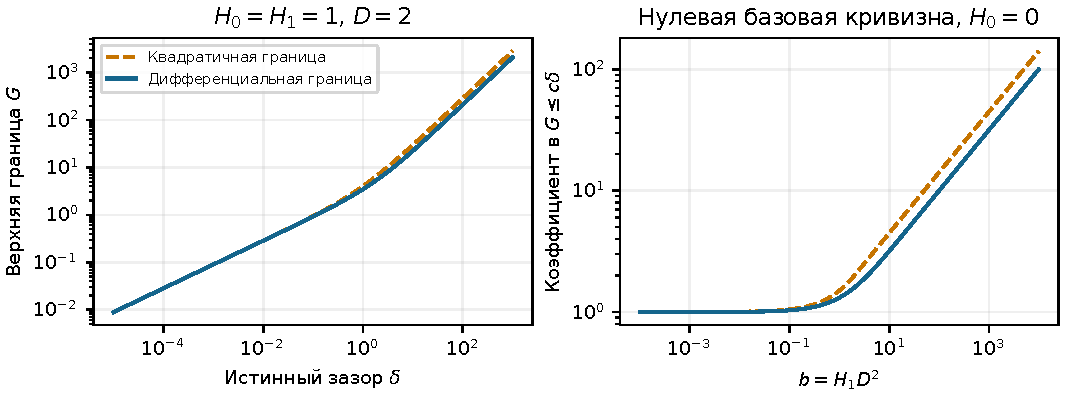
\includegraphics[width=\linewidth]{ru/figures/gap_geometry.pdf}
\caption{Поточечные теоретические границы. Дифференциальная огибающая
сохраняет изменение значения функции вдоль отрезка; сравнение с
фиксированной квадратичной моделью дано в~\eqref{eq:sharpbridge}.
При нулевой базовой кривизне точный линейный коэффициент равен
$\sqrt b\coth\sqrt b$. Это неравенства для класса функций,
а не траектории оптимизации или измерения времени.}
\label{fig:geometry}
\end{figure}

\begin{theorem}[Геометрическая сертификатная оценка AFW]\label{thm:geometric}
Предположим $H_0+H_1>0$ и~\eqref{eq:geometry}. Положим
\[
 J_*=\ceil{\log_2(U_0/\eta_\varepsilon)},\qquad
 P_*=\ceil{\log_2\max\{1,M/[2(H_0+H_1U_0)]\}}.
\]
При $0<\varepsilon<U_0$ тот же алгоритм достигает
$U_N\le\varepsilon$ за
\begin{equation}\label{eq:geometriccount}
 N\le2\ceil{P_*+(6+4H_0D^2/\kappa)J_*+8H_1D^2U_0/\kappa}
       +|S_0|-1
\end{equation}
обновлений. Формула~\eqref{eq:functioncount} остаётся верной.
Ни $H_0,H_1,\kappa$, ни $f_Q^*$ не являются входами алгоритма.
\end{theorem}
\begin{proof}
Анализируем фазы истинной ошибки $b_j/2<\delta_k\le b_j$ с
$b_j=U_0/2^j$ до достижения $\delta\le\eta_\varepsilon$.
Их положительные границы $C_j=2(H_0+H_1b_j)$ убывают не более
чем вдвое. Начальная истинная ошибка может пропустить фазы;
лемма~\ref{lem:lag} всё равно ограничивает запаздывающие обновления
числом $P_*+J_*$. На контролируемом хорошем шаге
\[
 f_k-f_{k+1}\ge\delta_k\min\{1/2,\kappa/(C_jD^2)\}
 >\min\{b_j/4,\kappa b_j/(2C_jD^2)\}.
\]
Для полного FW-шага используем $g\ge G\ge\delta$; для
необрезанного шага — условие~\eqref{eq:geometry}.
Бюджет фазы $b_j$ допускает не более
$5+4H_0D^2/\kappa+4H_1D^2b_j/\kappa$ контролируемых хороших
обновлений. Суммируем $\sum_{j<J_*}b_j<2U_0$, добавляем
запаздывающие обновления и применяем~\eqref{eq:dropcount}.
Теорема~\ref{lem:bridge} гарантирует, что к этому моменту фактический
сертификат уже прошёл порог.
\end{proof}

Для фиксированных задачи и инициализации зависимость от точности
логарифмическая. Явная фазовая цена $H_1$ пропорциональна $U_0$;
кроме того, $H_1$ входит в $J_*$ через~\eqref{eq:threshold}.
При выполнении геометрической гипотезы применимы обе AFW-оценки;
начальный вклад $U_0/\kappa$ означает, что геометрическая оценка
не всегда точнее выпуклой. Предполагать $H_0>0$ необязательно:
при $H_1>0$ границы положительны на положительных уровнях фаз.
Неаффинный пример — $f=t+(\max\{t,0\})^3$, $t=1/2-x$, на
$[-1/2,1/2]$ с $H_0=0,H_1=6$ и $\kappa=1/16$
(приложение~\ref{app:bridge}). На деле $H_0=0$ имеет более сильные
структурные следствия, доказанные далее без геометрического
неравенства~\eqref{eq:geometry}.
